\documentclass[border=4pt]{standalone}

\usepackage{tikz}

\definecolor{otblue}{HTML}{0072B2}
\definecolor{otorange}{HTML}{E69F00}
\definecolor{otteal}{HTML}{009E73}
\definecolor{otpurple}{HTML}{CC79A7}
\definecolor{otgray}{HTML}{5A5A5A}

\begin{document}
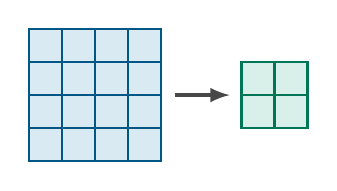
\begin{tikzpicture}[line width=0.9pt]
  \foreach \x in {0,1,2,3}{\foreach \y in {0,1,2,3}{\filldraw[draw=otblue!75!black, fill=otblue!15] ({\x*0.42},{\y*0.42}) rectangle +(0.42,0.42);}}
  \draw[otgray!80!black, line width=1.4pt, -latex] (1.85,0.84) -- (2.55,0.84);
  \foreach \x in {0,1}{\foreach \y in {0,1}{\filldraw[draw=otteal!75!black, fill=otteal!15] ({2.7+\x*0.42},{0.42+\y*0.42}) rectangle +(0.42,0.42);}}
\end{tikzpicture}
\end{document}
